\documentclass[letterpaper,11pt]{article}
\oddsidemargin -1.0cm \textwidth 17.5cm

\usepackage[utf8]{inputenc}
\usepackage[activeacute,spanish]{babel}
\usepackage{amsfonts,setspace}
\usepackage{amsmath}
\usepackage{amssymb, amsmath, amsthm}
\usepackage{comment}
\usepackage{amssymb}
\usepackage{dsfont}
\usepackage{anysize}
\usepackage{multicol}
\usepackage{enumerate}
\usepackage{graphicx}
\usepackage[left=1.5cm,top=2cm,right=1.5cm, bottom=1.7cm]{geometry}
\setlength\headheight{1.5em} 
\usepackage{fancyhdr}
\usepackage{multicol}
\usepackage{hyperref}
\usepackage{wrapfig}
\pagestyle{fancy}
\fancyhf{}
\renewcommand{\labelenumi}{\normalsize\bfseries P\arabic{enumi}.}
\renewcommand{\labelenumii}{\normalsize\bfseries (\alph{enumii})}
\renewcommand{\labelenumiii}{\normalsize\bfseries \roman{enumiii})}

\begin{document}

\fancyhead[L]{\itshape{Facultad de Ciencias F\'isicas y Matem\'aticas}}
\fancyhead[R]{\itshape{Universidad de Chile}}

\begin{minipage}{11.5cm}
    \begin{flushleft}
        \hspace*{-0.6cm}\textbf{FI1000-5 Introducción a la Física Clásica}\\
        \hspace*{-0.6cm}\textbf{Profesora:} Paulina Lira\\
        \hspace*{-0.6cm}\textbf{Auxiliares:} Alejandro Silva, Felipe Kaschel, Juan Cristobal Castro\\
    \end{flushleft}
\end{minipage}

\begin{picture}(2,3)
    \put(405,-5){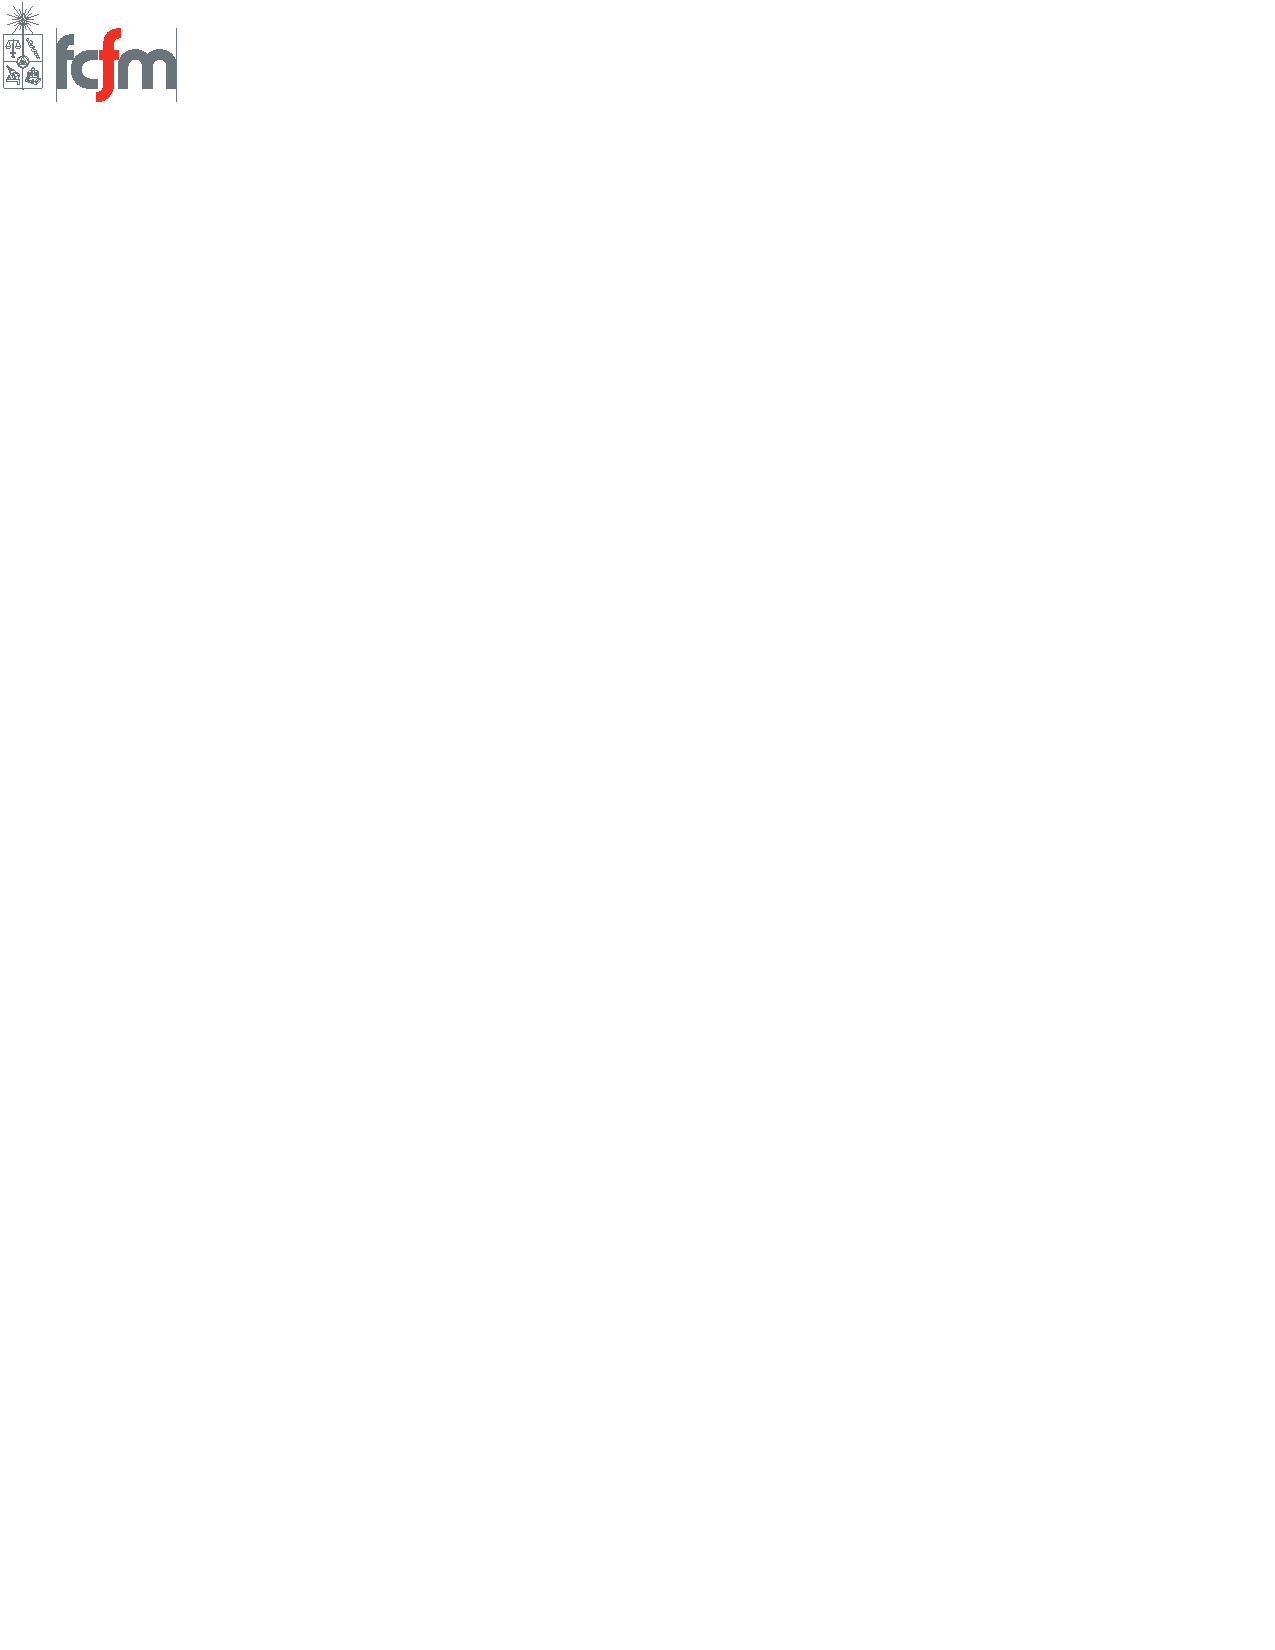
\includegraphics[scale=1.25]{2020-1/Imágenes/logo/fcfm2.pdf}}
\end{picture}

\begin{center}
	\LARGE \bf Auxiliar \#7: Fricción   \\
\end{center}

\vspace{-1cm}
\begin{enumerate}\setlength{\itemsep}{0.4cm}

\rfoot[]{pág. \thepage}

\item[]

\item Un automóvil de masa $m$ se traslada sobre una curva plana horizontal. Si el radio de la curva es $R$, el coeficiente de roce estático entre las llantas y el pavimento es $\mu_s$ y el coeficiente de roce cinético es $\mu_c$. Determine la rapidez máxima a la cual el automóvil completa una vuelta exitosamente.

\item Sea $\mu$ el coeficiente de roce estático entre la masa $m$ y el carro de masa $M$. ¿Cuál es la fuerza mínima que debe aplicarse al carro para que la masa $m$ no caiga?
\begin{figure}[h!]
    \centering
    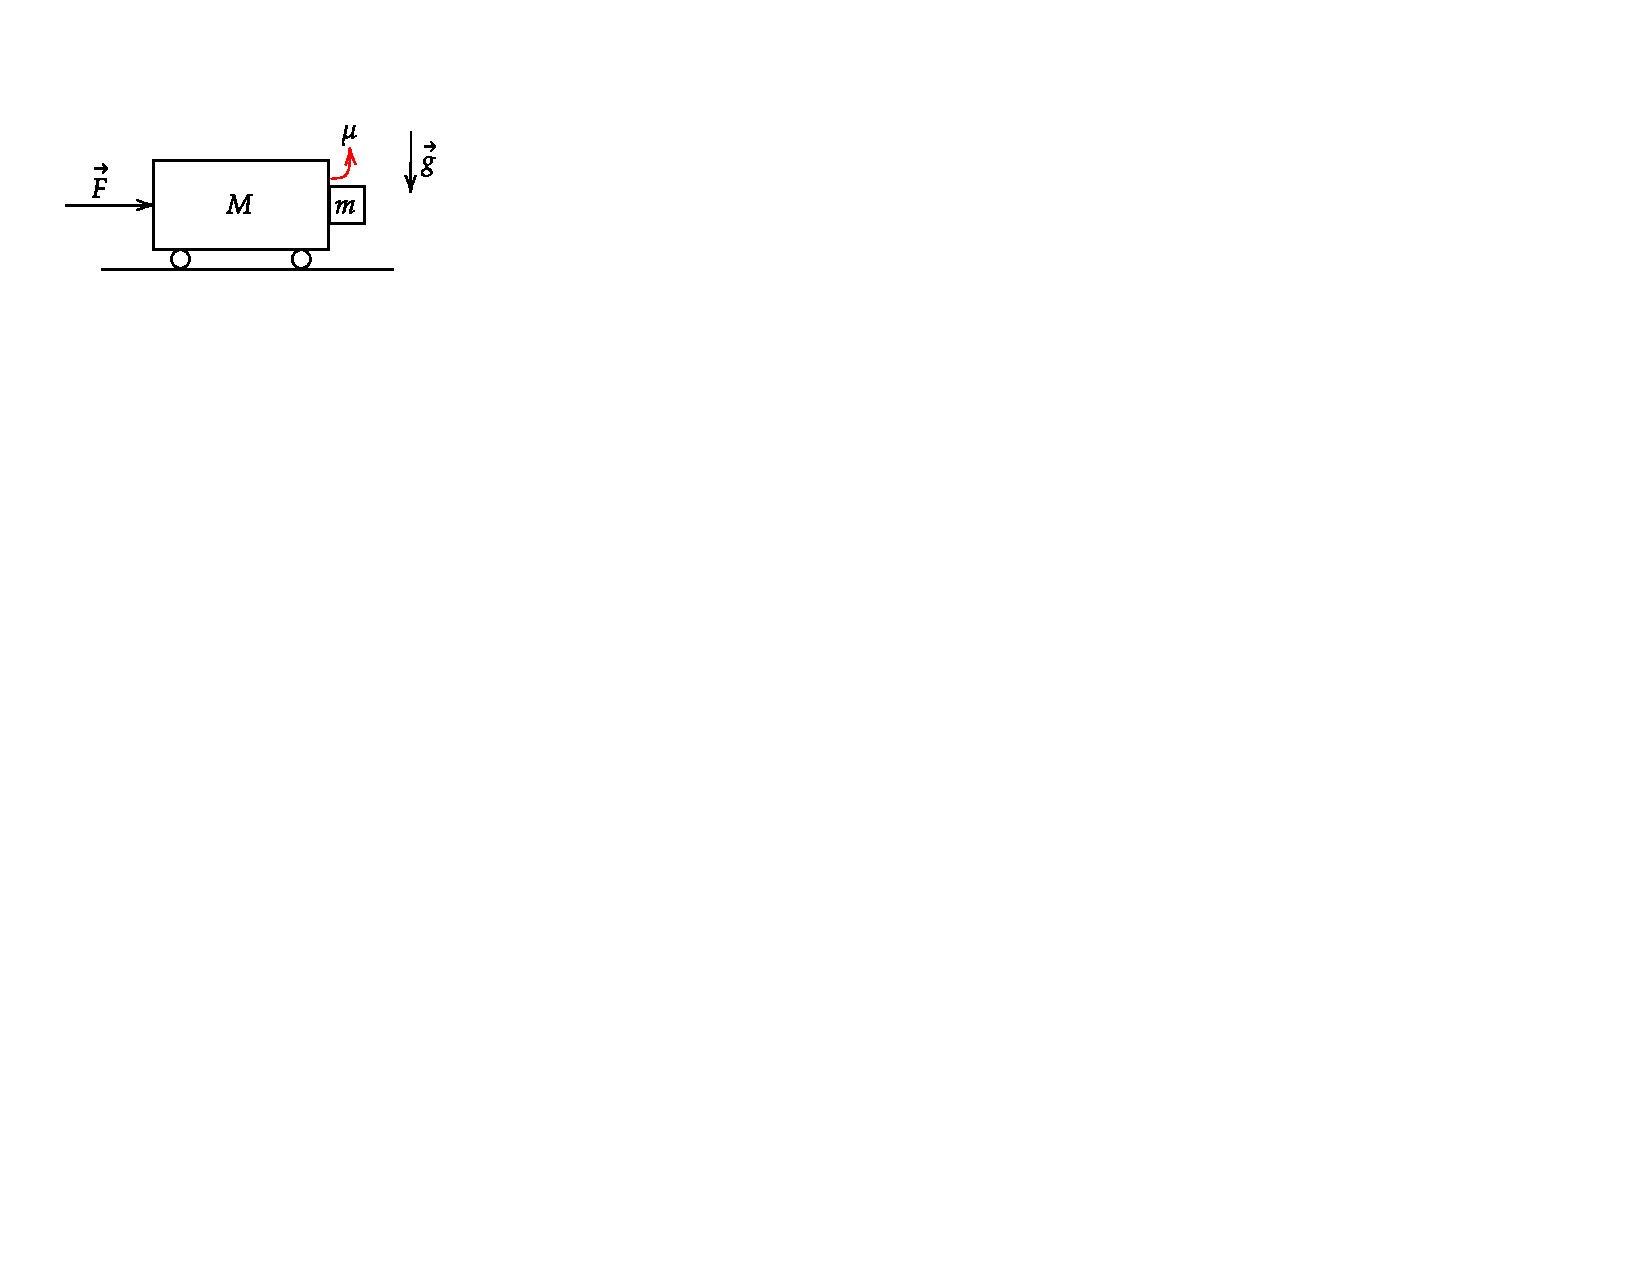
\includegraphics[scale = 0.8]{2020-1/Imágenes/aux7/carro.pdf}
\end{figure}

\item Sea un bloque de masa $m$ sobre dos cuñas de masas $M$. Las cuñas tienen una inclinación $\theta$ y entre las superficies de estas masas existe un coeficiente de roce cinemático $\mu$. El valor de $\mu$ es tal que el sistema no se encuentra en equilibrio, es decir, las cuñas se separan y el bloque baja. Entre las cuñas y el suelo el roce es nulo. Determine la aceleración del bloque $m$.

\begin{figure}[h!]
    \centering
    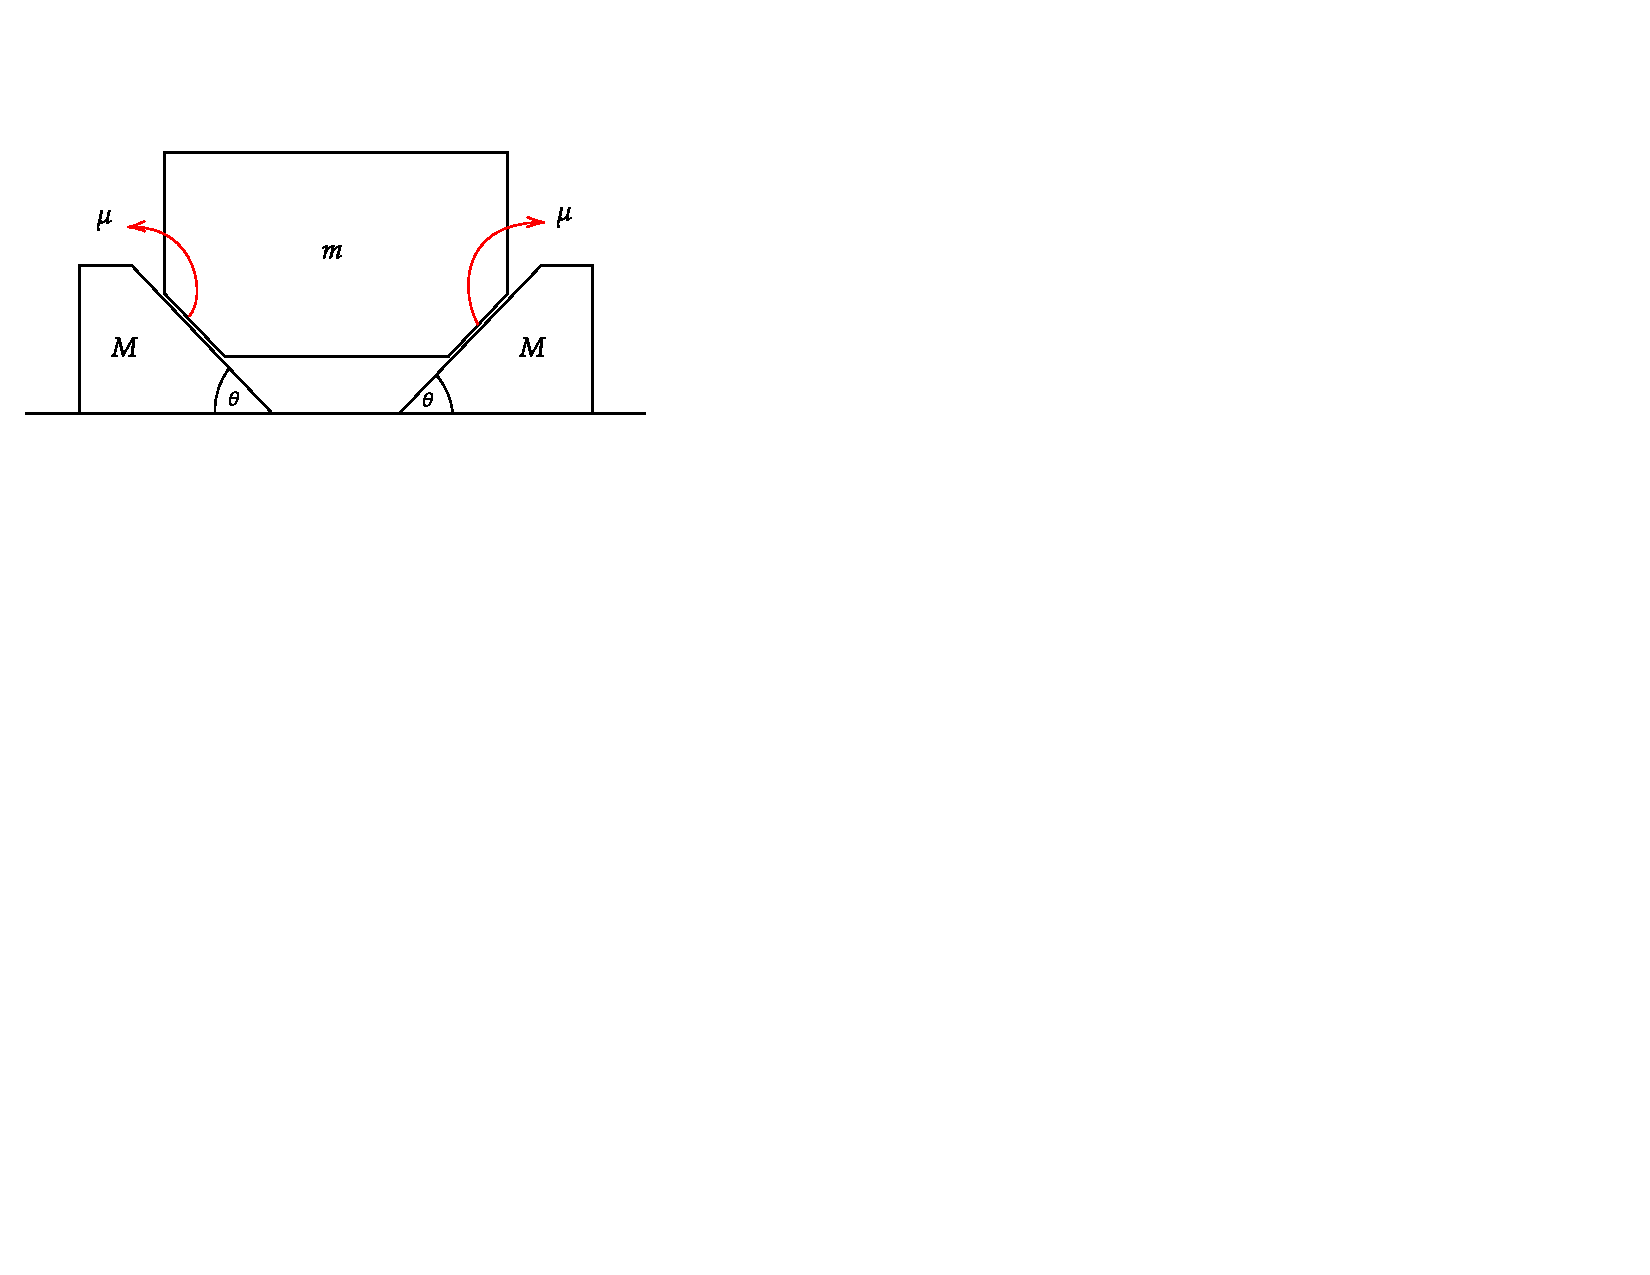
\includegraphics[scale=0.6]{2020-1/Imágenes/aux7/masa_cunias.pdf}
\end{figure}
\end{enumerate}
\end{document}